\documentclass[11pt]{article}
\usepackage[a4paper,margin=1in]{geometry}
\usepackage{amsmath,amssymb,amsthm}
\usepackage{tikz}
\usetikzlibrary{arrows.meta,calc}
\usepackage{xcolor}
\usepackage[hidelinks]{hyperref}
\hypersetup{pdftitle={Six unit sticks and the diameter of a hexagon},pdfauthor={Vamshi Jandhyala}}
\setlength{\parskip}{0.4em}
\setlength{\parindent}{0pt}

\newtheorem{theorem}{Theorem}
\newtheorem{lemma}{Lemma}
\newtheorem{proposition}{Proposition}
\newtheorem{corollary}{Corollary}
\theoremstyle{remark}
\newtheorem*{remark}{Remark}
\DeclareMathOperator{\conv}{conv}
\DeclareMathOperator{\diam}{diam}

\definecolor{inkblue}{RGB}{40,76,105}
\definecolor{softblue}{RGB}{226,235,243}
\definecolor{softgray}{RGB}{238,238,238}
\definecolor{rust}{RGB}{153,70,45}
\definecolor{pocket}{RGB}{246,226,205}

\title{Six unit sticks and the diameter of a hexagon}
\author{Vamshi Jandhyala}
\date{}

\begin{document}
\maketitle
\vspace{-2em}

\begin{abstract}
Join six sticks of length one, end to end, into a closed loop that does not cross itself.
How small can the loop be? We show that its diameter always exceeds $\sqrt2$, that
$\sqrt2$ is the best possible constant, and that it is never attained. In particular such a
hexagon fits neither in a unit square nor in a disk of radius $1/\sqrt2$, although a
pentagon and a heptagon fit in the unit square. This settles the first open case of a
parity question asked on MathOverflow. The proof uses only angles, convex hulls and one
triangle; its analytic and combinatorial steps are formally verified in Lean.
\end{abstract}

\section{The question}

Here is a puzzle to try before reading on. Can you build a closed polygon from six sticks
of length one, with no two sticks crossing or overlapping, that fits inside a $1\times1$
square? The square itself uses four sticks. Five sticks also fit: run three of them along
the bottom, right and left sides, and fold the remaining two into a spike that dips from
the top corners down to the point $(1/2,\,1-\sqrt3/2)$ (Figure~\ref{fig:examples}, left).

\begin{figure}[ht]
\centering
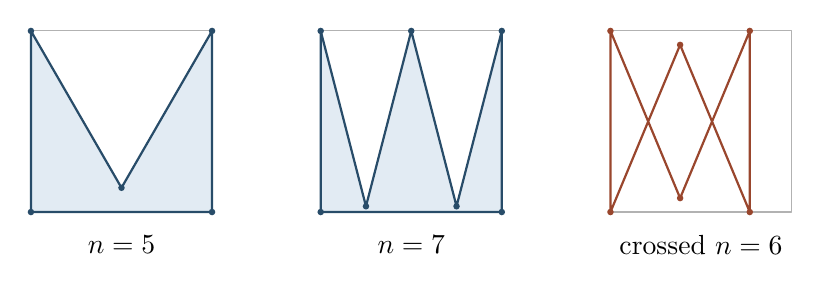
\begin{tikzpicture}[scale=2.3,line join=round]
  \draw[gray!60] (0,0) rectangle (1,1);
  \fill[softblue] (0,0)--(1,0)--(1,1)--(.5,{1-sqrt(3)/2})--(0,1)--cycle;
  \draw[thick,inkblue] (0,0)--(1,0)--(1,1)--(.5,{1-sqrt(3)/2})--(0,1)--cycle;
  \foreach \p in {(0,0),(1,0),(1,1),(.5,{1-sqrt(3)/2}),(0,1)}
    \fill[inkblue] \p circle (.018);
  \node at (.5,-.18) {$n=5$};
  \begin{scope}[xshift=1.6cm]
    \draw[gray!60] (0,0) rectangle (1,1);
    \fill[softblue] (0,0)--(1,0)--(1,1)--(.75,{1-sqrt(15)/4})--(.5,1)
      --(.25,{1-sqrt(15)/4})--(0,1)--cycle;
    \draw[thick,inkblue] (0,0)--(1,0)--(1,1)--(.75,{1-sqrt(15)/4})--(.5,1)
      --(.25,{1-sqrt(15)/4})--(0,1)--cycle;
    \foreach \p in {(0,0),(1,0),(1,1),(.75,{1-sqrt(15)/4}),(.5,1),(.25,{1-sqrt(15)/4}),(0,1)}
      \fill[inkblue] \p circle (.018);
    \node at (.5,-.18) {$n=7$};
  \end{scope}
  \begin{scope}[xshift=3.2cm]
    \draw[gray!60] (0,0) rectangle (1,1);
    \draw[thick,rust] (0,0)--(0,1)--({5/13},{1/13})--({10/13},1)
      --({10/13},0)--({5/13},{12/13})--cycle;
    \foreach \p in {(0,0),(0,1),({5/13},{1/13}),({10/13},1),({10/13},0),({5/13},{12/13})}
      \fill[rust] \p circle (.018);
    \node at (.5,-.18) {crossed $n=6$};
  \end{scope}
\end{tikzpicture}
\caption{Unit polygons in the unit square. The pentagon and heptagon are simple. The six
red sticks also have length one, but they cross.}
\label{fig:examples}
\end{figure}

The same trick gives every odd number of sticks from five on. For $2k+1$ sticks, put
$k$ equally spaced points on the top side and join consecutive ones through a
V-shaped dip of depth $\sqrt{1-1/(4(k-1)^2)}$; the figure shows $k=3$. Even numbers
seem to resist. Six sticks can be fitted into the square if they are allowed to cross
(Figure~\ref{fig:examples}, right), but every attempt to untangle them seems to push a
vertex out. JetfiRex asked on Mathematics Stack Exchange and MathOverflow whether this
is a law: must every simple unit polygon in the closed unit square, other than the
square's own boundary, have an odd number of sides~\cite{JetfiRexMSE,JetfiRexMO}?

The question is still open in general. Equilateral polygons of small diameter are well
studied among convex polygons, where one maximizes perimeter or width for a given
diameter~\cite{BinganeAudet}, and unit-distance drawings of cycles have been studied when
edges may cross~\cite{GMU}; the nonconvex, noncrossing case asked about here seems to be new.
This note settles six sides, and it does so with no square at all. The diameter of a polygon is the largest distance between two of its
points; the unit square has diameter $\sqrt2$, as does the disk of radius $1/\sqrt2$.

\begin{theorem}\label{thm:main}
Every simple unit hexagon has diameter greater than $\sqrt2$. The constant is sharp:
there are simple unit hexagons with diameter as close to $\sqrt2$ as we like.
\end{theorem}

\begin{corollary}\label{cor:boxes}
No simple unit hexagon fits in a closed square of side $1$ or in a closed disk of radius
$1/\sqrt2$. For every $\varepsilon>0$, one fits in a square of side $1+\varepsilon$ and in a
disk of radius $1/\sqrt2+\varepsilon$.
\end{corollary}

So in the square the obstruction for six sides is tight. The diameter version is the
stronger statement: it rules out every container of diameter $\sqrt2$ at once, the square
and the disk among them. The polygons approaching the bound
(Figure~\ref{fig:sharpness}) look like the pentagon above with its spike replaced by a
thin two-stick sliver.

\paragraph{The plan.} A diameter of at most $\sqrt2$ makes every angle of the polygon
sharp: at most a right angle on the inside at a convex corner, at least three right
angles at a reflex corner. Sharp angles are expensive. Two sharp turns in the same
direction swing the third stick back across the first, so turns must keep changing
sign, and the angle sum leaves room for only one or two reflex corners. Those reflex
corners must hide in ``pockets'' of the convex hull, and each pocket has to pay for
itself with reflex corners. Counting what is left for the hull leads, in each case, to
one of three small configurations, each excluded by a short lemma.

\section{Sharp turns}

A polygon is \emph{simple} if its vertices are distinct, nonadjacent edges are disjoint,
and adjacent edges meet only at their shared vertex. A \emph{unit polygon} has all
edges of length one. Orient every polygon counterclockwise. At each vertex the two
edges make a \emph{smaller angle} $\theta\in(0,\pi]$; the interior angle is $\theta$ at a
\emph{convex} vertex and $2\pi-\theta$ at a \emph{reflex} one, and the turn there is
$\pi-\theta$ to the left or to the right.

\emph{Small diameter means sharp corners.} If $D$ is the diameter, a vertex whose
neighbors are at distance $d$ has, by the law of cosines,
\begin{equation}\label{eq:cosine}
  d^2 = 2-2\cos\theta .
\end{equation}
In words: the farther apart the neighbors, the more open the angle. With
$d\le D\le\sqrt2$ this gives $\cos\theta\ge0$, so
\begin{equation}\label{eq:angles}
  0<\theta\le\frac{\pi}{2}
\end{equation}
at every vertex of a unit polygon of diameter at most $\sqrt2$. (A zero angle would make
the neighbors coincide.) Every convex interior angle is at most $\pi/2$, and every reflex
interior angle is at least $3\pi/2$.

\emph{Two sharp turns in the same direction are impossible.} Try it: walk along a unit
stick, turn left by more than a right angle, walk again, and turn left sharply once more.
The third stick heads back across the first (Figure~\ref{fig:turns}). Boilley made this
observation in the Mathematics Stack Exchange discussion~\cite{Boilley}; here is a sharp
form of it.

\begin{figure}[ht]
\centering
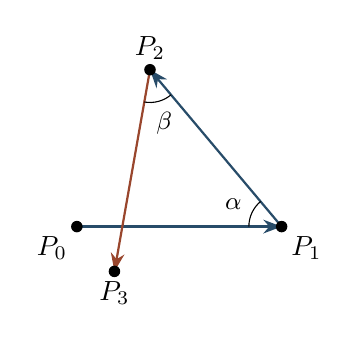
\begin{tikzpicture}[scale=2.6,>=Stealth,line join=round]
  \coordinate (P0) at (0,0);
  \coordinate (P1) at (1,0);
  \coordinate (P2) at ({1-cos(50)},{sin(50)});
  \coordinate (P3) at ({1-cos(50)+cos(100)},{sin(50)-sin(100)});
  \draw[thick,inkblue,->] (P0)--(P1);
  \draw[thick,inkblue,->] (P1)--(P2);
  \draw[thick,rust,->] (P2)--(P3);
  \draw (P1) ++(180:.16) arc (180:130:.16);
  \node[font=\small] at ($(P1)+(155:.26)$) {$\alpha$};
  \draw (P2) ++(-50:.16) arc (-50:-100:.16);
  \node[font=\small] at ($(P2)+(-75:.27)$) {$\beta$};
  \foreach \p/\pos in {P0/below left,P1/below right,P2/above,P3/below}
    {\fill (\p) circle (.8pt);}
  \node[below left] at (P0) {$P_0$};
  \node[below right] at (P1) {$P_1$};
  \node[above] at (P2) {$P_2$};
  \node[below] at (P3) {$P_3$};
\end{tikzpicture}
\caption{Two left turns with smaller angles $\alpha=\beta=50^\circ$. The third stick
crosses the first.}
\label{fig:turns}
\end{figure}

\begin{lemma}[Adjacent turns]\label{lem:turns}
In a simple unit polygon with at least four sides, let two consecutive vertices turn the
same way, with smaller angles $\alpha,\beta\in(0,\pi/2]$. Then
\[
  \max(2\alpha+\beta,\ \alpha+2\beta)>\pi,
\]
and consequently $\alpha+\beta>\pi/2$ and $\max(\alpha,\beta)>\pi/3$.
\end{lemma}

\begin{proof}
Reflecting if necessary, both turns are to the left. Place the three edges as
\[
  P_0=(0,0),\quad P_1=(1,0),\quad P_2=(1-\cos\alpha,\ \sin\alpha),\quad
  P_3=P_2+\bigl(\cos(\alpha+\beta),\ -\sin(\alpha+\beta)\bigr).
\]
Suppose $2\alpha+\beta\le\pi$ and $\alpha+2\beta\le\pi$. Then $\alpha+\beta<\pi$, and
$\alpha\le\min\bigl(\alpha+\beta,\ \pi-(\alpha+\beta)\bigr)\le\pi/2$; since
$\sin(\alpha+\beta)=\sin\bigl(\pi-(\alpha+\beta)\bigr)$ and the sine increases on $[0,\pi/2]$, this gives
$\sin\alpha\le\sin(\alpha+\beta)$, and in the same way $\sin\beta\le\sin(\alpha+\beta)$. The point at parameter
$s=\sin\alpha/\sin(\alpha+\beta)\in[0,1]$ along $P_2P_3$ has height zero, and a short computation
with the subtraction formula for the sine puts it at
\[
  x=1-\frac{\sin\beta}{\sin(\alpha+\beta)}\in[0,1].
\]
So the third edge meets the first, which is forbidden in a simple polygon with at least
four sides (the two edges are not adjacent). This proves the inequality. Since
$\alpha,\beta\le\pi/2$, the larger of the two terms is at most $\alpha+\beta+\pi/2$, giving
$\alpha+\beta>\pi/2$; and if both angles were at most $\pi/3$, both terms would be at most
$\pi$.
\end{proof}

The next lemma says that a short unit path with sharp corners cannot fold its middle
vertices inside its own hull.

\begin{lemma}[Projection]\label{lem:projection}
Let $X_0,X_1,X_2,X_3$ be distinct points in the plane with
$|X_0X_1|=|X_1X_2|=|X_2X_3|=1$ and
$|X_0X_2|\le\sqrt2$. Then $X_1\notin\conv(X_0,X_2,X_3)$. Symmetrically, if
$|X_1X_3|\le\sqrt2$ then $X_2\notin\conv(X_0,X_1,X_3)$.
\end{lemma}

\begin{proof}
Measure every point by its component along $b=X_1-X_2$, starting from $X_2$:
$f(Y)=(Y-X_2)\cdot b$. Then $f(X_1)=1$ and $f(X_2)=0$. Expanding
$|X_3-X_1|^2=|(X_3-X_2)-b|^2=2-2f(X_3)$ shows $f(X_3)<1$, because $X_3\ne X_1$. In the
same way $|X_0-X_1|=1$ gives $f(X_0)=|X_0-X_2|^2/2\le1$. A convex combination of
$X_0,X_2,X_3$ therefore has $f\le1$, with equality only when all the weight sits on
$X_0$; but $X_0\ne X_1$. The second statement is the first for the reversed path.
\end{proof}

\begin{lemma}[Four hull edges]\label{lem:fourhull}
Let $P_0,\dots,P_4$ be distinct points on the boundary of their convex hull, in
counterclockwise order, with $|P_iP_{i+1}|=1$ for $i=0,1,2,3$. Then the interior angles
$\alpha,\beta,\gamma$ of the hull at $P_1,P_2,P_3$ cannot all lie in $(0,\pi/2]$.
\end{lemma}

The endpoints $P_0,P_4$ may lie in the middle of a hull side; the lemma allows that.

\begin{proof}
Suppose $\alpha,\beta,\gamma\in(0,\pi/2]$ and put $S=\alpha+\beta+\gamma$. Going once around the
closed polygon $P_0P_1P_2P_3P_4$, the five turns add up to $2\pi$. The three middle turns
give $3\pi-S$, and the turns at $P_0,P_4$ are nonnegative. They cannot both be zero:
then $P_3,P_4,P_0,P_1$ would lie on a line in this order, and $|P_3P_1|=2+|P_4P_0|>2$,
although the path $P_3P_2P_1$ has length two. Hence $S>\pi$.

Now place $P_0=(0,0)$ and $P_1=(1,0)$. The four edges point in the directions $0$,
$\pi-\alpha$, $2\pi-\alpha-\beta$ and $3\pi-S$, so
\[
  P_4=\bigl(1-\cos\alpha+\cos(\alpha+\beta)-\cos S,\ \ \sin\alpha-\sin(\alpha+\beta)+\sin S\bigr).
\]
Convexity at $P_0$ and at $P_4$ says that the cross products of incoming and outgoing
edges there are nonnegative. At $P_0$ this cross product is the height of $P_4$; at
$P_4$ a short expansion with the subtraction formula gives a mirror image:
\begin{equation}\label{eq:K}
  K_0=\sin\alpha-\sin(\alpha+\beta)+\sin S,\qquad K_4=\sin\gamma-\sin(\beta+\gamma)+\sin S.
\end{equation}
Swapping $\alpha$ and $\gamma$ exchanges them, so we may assume $\gamma\le\alpha$ and show
$K_4<0$. Since $\pi<S\le3\pi/2$, $\sin S<0$.

If $2\gamma+\beta\le\pi$, then $\sin\gamma\le\sin(\beta+\gamma)$, as in Lemma~\ref{lem:turns},
and $K_4<0$. If $2\gamma+\beta>\pi$, then $\pi<2\gamma+\beta\le S\le3\pi/2$, where the sine
decreases, so
\[
  K_4\le\sin\gamma-\sin(\beta+\gamma)+\sin(2\gamma+\beta)
  =4\sin\frac{\gamma}{2}\,\cos\frac{\beta+\gamma}{2}\,\cos\Bigl(\gamma+\frac{\beta}{2}\Bigr).
\]
The three factors are positive, nonnegative and negative, so $K_4\le0$, with equality
only if $\beta+\gamma=\pi$. That forces $\alpha=\beta=\gamma=\pi/2$: three right angles, and then
$P_4=P_0$, which is excluded.
\end{proof}

\section{A triangle with two unit sides}

Here is a container that holds no unit polygon at all, apart from itself.

\begin{proposition}\label{prop:triangle}
Let $T$ be a nondegenerate triangle with two sides of length one. Then $T$ contains no
simple unit polygon with four or more sides.
\end{proposition}

\begin{figure}[ht]
\centering
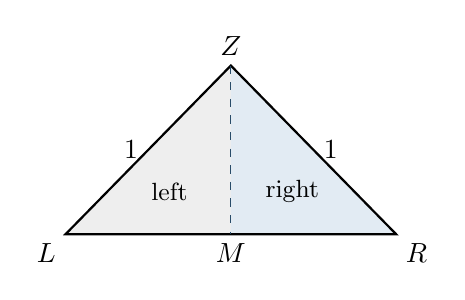
\begin{tikzpicture}[scale=3.0]
  \coordinate (L) at (-.7,0);
  \coordinate (R) at (.7,0);
  \coordinate (Z) at (0,{sqrt(.51)});
  \coordinate (M) at (0,0);
  \fill[softgray] (L)--(Z)--(M)--cycle;
  \fill[softblue] (M)--(Z)--(R)--cycle;
  \draw[thick] (L)--node[left] {$1$}(Z)--node[right] {$1$}(R)--cycle;
  \draw[dashed,inkblue] (Z)--(M);
  \foreach \p/\pos in {L/below left,R/below right,Z/above,M/below}
    \node[\pos] at (\p) {$\p$};
  \node[font=\small] at (-.26,.18) {left};
  \node[font=\small] at (.26,.18) {right};
\end{tikzpicture}
\caption{Each closed half has diameter one, attained only by its sloping side. A unit edge
that avoids $Z$ must therefore cross from one open half to the other.}
\label{fig:triangle}
\end{figure}

\begin{proof}
Put $L=(-a,0)$, $R=(a,0)$, $Z=(0,h)$ with $0<a<1$, $h>0$, $a^2+h^2=1$. The median
$ZM$ cuts $T$ into two closed halves (Figure~\ref{fig:triangle}). Four facts about
distances do all the work.
\begin{enumerate}
\item[(a)] Two points of the left half differ by at most $a$ horizontally and at most $h$
vertically, so their distance is at most $\sqrt{a^2+h^2}=1$. Equality needs both
differences to be extreme, and the only such pair is $L,Z$. The right half is the mirror
image.
\item[(b)] A median point $(0,y)$ with $y<h$ is at squared distance $a^2+y^2<1$ from $L$
and $R$ and $(h-y)^2<1$ from $Z$; distance to a point of $T$ is largest at a corner, so it
has no point of $T$ at distance one.
\item[(c)] Every point of $T$ is within distance one of $Z$, and only $L,R$ are at distance
exactly one.
\item[(d)] Hence a unit segment in $T$ that avoids $Z$ joins a point with $x<0$ to a point
with $x>0$.
\end{enumerate}
Label each vertex of a unit polygon in $T$, other than $Z$, \emph{left} or \emph{right}
by the sign of its $x$-coordinate. By (d), along any run of vertices avoiding $Z$ the
labels alternate. The two neighbors of such a vertex are within distance one of each
other: either both carry the opposite label, so lie in one half, or one of them is $Z$.
By~\eqref{eq:cosine}, its smaller angle is at most $\pi/3$, and Lemma~\ref{lem:turns} then
says that consecutive turns change sign. So along any run avoiding $Z$, both the labels
and the convex/reflex types alternate, and the truth of the statement
\[
  \text{``this vertex is convex''}\iff\text{``this vertex is left''}
\]
never changes. That is the whole argument; it remains to find two vertices that disagree.

If the polygon avoids $Z$, take a leftmost and a rightmost vertex. Both are convex, since
a vertex on a supporting line of the polygon cannot be reflex, and the statement is true
at the first and false at the second. If the polygon passes through $Z$, then by (c) the
neighbors of $Z$ are $L$ and $R$, both convex as corners of $T$; on the rest of the
polygon, a run from $L$ to $R$ avoiding $Z$, the statement is true at $L$ and false at
$R$. Either way we have a contradiction.
\end{proof}

\begin{remark}
A unit triangle in $T$ is possible only when $|LR|=1$ and the triangle is $T$ itself. No
diameter bound is assumed in the proposition.
\end{remark}

\section{Pockets}

Let $P$ be a simple polygon and $H$ its convex hull. Call a vertex of $P$ a \emph{contact}
if it lies on the boundary of $H$; corners of $H$ are contacts, and so are vertices in
the middle of a hull side. A reflex vertex is never a contact, because $P$ lies on one
side of every supporting line of $H$.

\begin{figure}[ht]
\centering
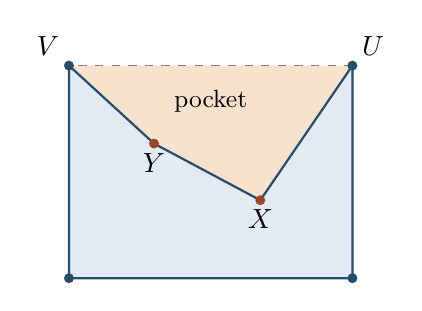
\begin{tikzpicture}[scale=0.9,line join=round]
  \coordinate (A) at (0,0);
  \coordinate (B) at (4,0);
  \coordinate (C) at (4,3);
  \coordinate (X) at (2.7,1.1);
  \coordinate (Y) at (1.2,1.9);
  \coordinate (D) at (0,3);
  \fill[softblue] (A)--(B)--(C)--(X)--(Y)--(D)--cycle;
  \fill[pocket] (C)--(X)--(Y)--(D)--cycle;
  \draw[dashed,gray] (C)--(D);
  \draw[thick,inkblue] (A)--(B)--(C)--(X)--(Y)--(D)--cycle;
  \foreach \p in {A,B,C,D} \fill[inkblue] (\p) circle (2pt);
  \foreach \p in {X,Y} \fill[rust] (\p) circle (2pt);
  \node[above right] at (C) {$U$};
  \node[above left] at (D) {$V$};
  \node[below] at (X) {$X$};
  \node[below] at (Y) {$Y$};
  \node[font=\small] at (2.0,2.5) {pocket};
\end{tikzpicture}
\caption{A pocket: the polygon path $U,X,Y,V$ between consecutive contacts leaves the hull
boundary, and with the hull segment $VU$ it bounds a region outside the polygon.}
\label{fig:pocket}
\end{figure}

\begin{lemma}[Pockets]\label{lem:pockets}
The contacts occur in the same cyclic order along $P$ as along the boundary of $H$.
Between two contacts $U,V$ that are consecutive along $P$, the path of $P$ either is the
hull segment $UV$ or has all its intermediate vertices inside $H$; in the second case it
contains a reflex vertex. Different such paths have no intermediate vertex in common.
\end{lemma}

\begin{proof}
We use two standard consequences of the Jordan curve theorem; see Toussaint's
survey~\cite{Toussaint} for this language of pockets and lids. First, two disjoint arcs
inside a convex region cannot join interleaved pairs of boundary points, so the polygon
visits the contacts in hull order. In particular consecutive contacts $U,V$ lie on a
common hull side, because every corner of $H$ is a contact. Second, if the path from $U$
to $V$ leaves that side, it bounds together with the segment $VU$ a simple polygon, the
\emph{pocket}, lying outside $P$ (Figure~\ref{fig:pocket}). Traversed as $U\to\dots\to V\to U$,
the pocket is clockwise, because $P$ lies to the left of its own boundary. Its turns add up
to $-2\pi$; the turns at $U$ and $V$ are greater than $-\pi$, so some intermediate turn is
negative. Intermediate turns are turns of $P$, so that vertex is reflex in $P$.
\end{proof}

When the diameter is at most $\sqrt2$, a pocket has to pay for its size.

\begin{lemma}[Cost of a pocket]\label{lem:cost}
Let $P$ be a simple unit polygon of diameter at most $\sqrt2$, and let a pocket have $k$
intermediate vertices, $r$ of them reflex in $P$. Then $r>k/3$. If $k=2$, both
intermediate vertices are reflex.
\end{lemma}

\begin{proof}
The pocket has $k+2$ vertices, so its interior angles sum to $k\pi$. At a vertex convex in
$P$ the pocket sees the outside angle $2\pi-\theta\ge3\pi/2$, by~\eqref{eq:angles}. All its
other angles are positive, so $\tfrac{3\pi}{2}(k-r)<k\pi$, which is $r>k/3$.

For $k=2$, write the path as $U,X,Y,V$. Lemma~\ref{lem:projection} applies in both
directions, so neither $X$ nor $Y$ is in the convex hull of the other three points; and
neither $U$ nor $V$ is, since $X,Y$ lie strictly on one side of the hull line through $U$
and $V$. Four points in convex position bound exactly one simple quadrilateral, the
convex one, so the pocket is convex. All its turns have the same sign, the clockwise one,
and in particular $X$ and $Y$ are reflex in $P$.
\end{proof}

\section{Proof of the theorem}

Suppose a simple unit hexagon has diameter at most $\sqrt2$. Its interior angles add up to
$4\pi$. Six convex angles of at most $\pi/2$ add up to at most $3\pi$, and three reflex angles
of at least $3\pi/2$ already exceed $4\pi$; so there are one or two reflex vertices.

\emph{One reflex vertex.} The reflex vertex is not a contact, so it sits in a pocket, and
by Lemma~\ref{lem:pockets} every pocket needs a reflex vertex of its own. So there is exactly
one pocket, and it holds every vertex that is not a contact. Let $m\in\{3,4,5\}$ be the number of contacts.
\begin{itemize}
\item $m=5$: the other four hull steps are polygon edges, forming a chain $P_0,\dots,P_4$
as in Lemma~\ref{lem:fourhull}. Its middle angles are angles of the hexagon, hence in
$(0,\pi/2]$; impossible.
\item $m=4$: the pocket has two intermediate vertices, both reflex by Lemma~\ref{lem:cost};
impossible.
\item $m=3$: the hull is a triangle whose two non-pocket sides are edges of the hexagon,
so it has two unit sides, and Proposition~\ref{prop:triangle} excludes it.
\end{itemize}

\emph{Two reflex vertices.} Call their smaller angles $\beta_1,\beta_2\le\pi/2$. The angle sum
gives
\[
  (\text{sum of the four convex angles})+(2\pi-\beta_1)+(2\pi-\beta_2)=4\pi,
\]
so the four convex angles add up to $\beta_1+\beta_2\le\pi$. If the reflex vertices are adjacent
or opposite, the convex vertices split into two disjoint adjacent pairs, and by
Lemma~\ref{lem:turns} each pair adds up to more than $\pi/2$: too much. The remaining
arrangement is, up to relabeling,
\[
  A,B,C,D,E,F\quad\text{with $B,D$ reflex and $A,C,E,F$ convex.}
\]
The corners of the hull are among $A,C,E,F$, and there are three or four of them.

\emph{Three corners.} One of $A,C,E,F$ is not a corner.
If it is $C$, the hull is the triangle $AEF$, and $EF$, $FA$ are unit sides; this is
excluded by Proposition~\ref{prop:triangle}. If it is $A$, the hull is $\conv(C,E,F)$, but
Lemma~\ref{lem:projection} for the path $C,D,E,F$ puts $D$ outside it. If it is
$E$, the same lemma for $F,A,B,C$ puts $B$ outside the hull $\conv(F,A,C)$. If it is $F$, then $F$
lies in the triangle $ACE$, which is counterclockwise. Writing $F=\lambda A+\mu C+\nu E$ with
nonnegative weights, the turn at $F$ along $E,F,A$ has cross product
$-\mu\cdot(\text{orientation of }ACE)\le0$: it turns right or goes straight, against the
convexity of $F$ and~\eqref{eq:angles}.

\emph{Four corners.} The hull is the quadrilateral $ACEF$, counterclockwise by
Lemma~\ref{lem:pockets}. Its diagonal
$CF$ splits it into the triangles $FAC$ and $CEF$. Lemma~\ref{lem:projection} for the paths
$F,A,B,C$ and $C,D,E,F$ gives $B\notin\conv(F,A,C)$ and $D\notin\conv(C,E,F)$. Since $B$ and
$D$ are inside the hull, $B$ lies strictly on the $E$ side of $CF$, and $D$ strictly on the
$A$ side. Seen from $C$, the rays therefore come in the order $CE$, $CB$, $CF$, $CD$, $CA$
(Figure~\ref{fig:hull}): going $B\to C\to D$, the path turns right at $C$, so $C$ is reflex.
This contradiction completes the proof of the bound $\diam>\sqrt2$.

\begin{figure}[ht]
\centering
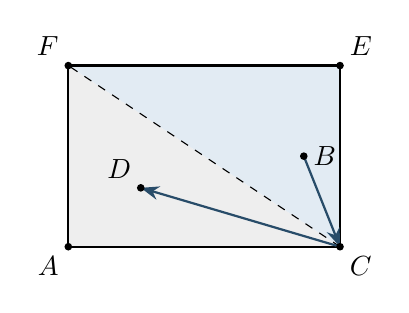
\begin{tikzpicture}[scale=1.15,>=Stealth]
  \coordinate (A) at (0,0);
  \coordinate (C) at (3,0);
  \coordinate (E) at (3,2);
  \coordinate (F) at (0,2);
  \coordinate (B) at (2.6,1);
  \coordinate (D) at (.8,.65);
  \fill[softgray] (F)--(A)--(C)--cycle;
  \fill[softblue] (C)--(E)--(F)--cycle;
  \draw[thick] (A)--(C)--(E)--(F)--cycle;
  \draw[dashed] (C)--(F);
  \draw[thick,inkblue,->] (B)--(C);
  \draw[thick,inkblue,->] (C)--(D);
  \foreach \p/\pos in {A/below left,C/below right,E/above right,F/above left,B/right,D/above left}
    {\fill (\p) circle (1.2pt);\node[\pos] at (\p) {$\p$};}
\end{tikzpicture}
\caption{The four-corner case. $B$ must sit in the blue triangle and $D$ in the gray one, so
the path $B\to C\to D$ turns right at $C$. Only the order of the rays is to scale.}
\label{fig:hull}
\end{figure}

\section{Sharpness}

It remains to build hexagons whose diameter approaches $\sqrt2$. Start from the unit square
$A=(0,0)$, $B=(1,0)$, $C=(1,1)$ and the point $(0,1)$, and replace the left side by a thin
two-stick sliver. For $0<t<1/2$ put
\[
  D=\Bigl(\frac{2t^2}{1+t^2},\ 1+\frac{2t}{1+t^2}\Bigr),\qquad
  E=D+\Bigl(\frac35,\,-\frac45\Bigr),
\]
so $D$ is on the unit circle about $C$, slightly above the square, and $E$ is one unit
from $D$, inside the square. Let $F$ be the intersection of the unit circles about $A$
and $E$ that lies to the left of $AE$:
\[
  F=\frac{E}{2}+k\,(-E_y,\ E_x),\qquad k=\sqrt{\frac{1}{|E|^2}-\frac14}.
\]
All six edges of $ABCDEF$ have length one (Figure~\ref{fig:sharpness}).

\begin{figure}[ht]
\centering
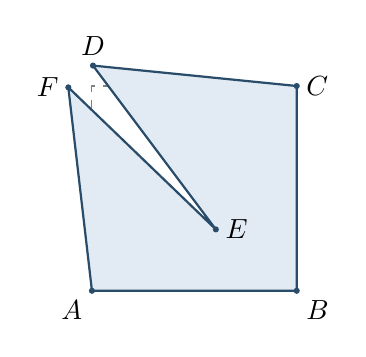
\begin{tikzpicture}[scale=2.6,line join=round]
 \pgfmathsetmacro{\dx}{2/401}
 \pgfmathsetmacro{\dy}{441/401}
 \pgfmathsetmacro{\ex}{\dx+.6}
 \pgfmathsetmacro{\ey}{\dy-.8}
 \pgfmathsetmacro{\kk}{sqrt(1/(\ex*\ex+\ey*\ey)-.25)}
 \pgfmathsetmacro{\fx}{\ex/2-\kk*\ey}
 \pgfmathsetmacro{\fy}{\ey/2+\kk*\ex}
 \coordinate (A) at (0,0);\coordinate (B) at (1,0);
 \coordinate (C) at (1,1);\coordinate (D) at (\dx,\dy);
 \coordinate (E) at (\ex,\ey);\coordinate (F) at (\fx,\fy);
 \draw[dashed,gray] (0,0) rectangle (1,1);
 \fill[softblue] (A)--(B)--(C)--(D)--(E)--(F)--cycle;
 \draw[thick,inkblue] (A)--(B)--(C)--(D)--(E)--(F)--cycle;
 \foreach \p/\pos in {A/below left,B/below right,C/right,D/above,E/right,F/left}
  {\fill[inkblue] (\p) circle (.015);\node[\pos] at (\p) {$\p$};}
\end{tikzpicture}
\caption{The hexagon at $t=1/20$, with the unit square dashed. As $t\to0$, $D$ and $F$
both tend to the corner $(0,1)$ and $E$ to $(3/5,1/5)$.}
\label{fig:sharpness}
\end{figure}

\emph{It is simple.} One identity carries the argument:
\begin{equation}\label{eq:sign}
  2E_y-|E|^2=\frac{16\,t\,(1-2t)}{5\,(1+t^2)} .
\end{equation}
The left side compares the height of $E$ with its squared distance from $A$; the right
side is positive on $0<t<1/2$. Squaring the two terms of $F_x=E_x/2-kE_y$ shows that
\eqref{eq:sign} is equivalent to $F_x<0$. Also $F_y>0$, and $|F|=1$ gives $F_y<1$. With
$0<D_x<2/5$, $D_y>1$ and $0<E_x,E_y<1$, every pair of nonadjacent edges is separated by
one of the lines $y=0$, $x=1$, $y=1$, $x=0$: for example $CD$ lies on or above $y=1$
while $EF$ and $FA$ lie below it, and $DE$ lies right of $x=0$ while $FA$ does not. The
turn cross products at $A,B,C,D,F$ are
\[
  F_y,\quad 1,\quad \frac{1-t^2}{1+t^2},\quad \frac{2(1-2t)(t+2)}{5(1+t^2)},\quad
  E_xF_y-E_yF_x,
\]
all positive, and at $E$ it is $\tfrac35(F_y-D_y)+\tfrac45(F_x-D_x)<0$. No turn is zero, so
adjacent edges meet only at their shared vertex.

\emph{Its diameter tends to $\sqrt2$.} As $t\to0$ the vertices tend to the four corners of
the unit square and $E_0=(3/5,1/5)$, with $k\to3/2$ and $F\to(0,1)$. Every pairwise
distance tends to at most $\sqrt2$, so the diameter tends to $\sqrt2$, and with the first
part this proves Theorem~\ref{thm:main}. The same limit puts the hexagon in a box of side
tending to one and within distance tending to $1/\sqrt2$ of $(1/2,1/2)$; since squares and
disks are convex, they contain the hexagon once they contain its vertices. This proves
Corollary~\ref{cor:boxes}.

\section{Eight sticks and beyond}

The square question for eight or more sides is open. The same tools go some way. In the unit square the diameter is at most $\sqrt2$, so all the lemmas apply, and for an
octagon the angle sum allows two or three reflex vertices. With two, the
hull perimeter is at most four, so fewer than four hull steps can be unit edges, and the
pocket lemmas leave one configuration.

\begin{proposition}\label{prop:octagon}
If a simple unit octagon in the closed unit square has exactly two reflex vertices, its
hull is a quadrilateral with three sides that are edges of the octagon, and the fourth
side closes a single pocket holding both reflex vertices and two convex ones.
\end{proposition}

\begin{proof}
Let $m$ count contacts and $q$ pockets. Each pocket holds a reflex vertex, so $q\le2$, and
the $m-q$ hull steps outside pockets are unit edges. The hull has perimeter at most four
(project each side onto the axes) and each pocket lid has positive length, so $m-q\le3$.
If $q=2$, each pocket has one reflex vertex, so $k<3$ by Lemma~\ref{lem:cost}, and $k\ne2$
by its second part; then $k=1$ for both, $m=6$ and $m-q=4$, a contradiction. So $q=1$ and
$m\le4$. If $m=3$, the hull is a triangle with two unit sides, excluded by
Proposition~\ref{prop:triangle}. When $m=4$, no contact lies in the middle of a hull side:
at the two middle contacts that would be a straight angle, against~\eqref{eq:angles}, and
at an end contact the hull would be a triangle with two unit sides.
\end{proof}

We do not know how to finish this case, nor the case of three reflex vertices. Boilley
suggested~\cite{Boilley} that the disk of radius $1/\sqrt2$ should behave like the square.
A stronger guess is that Theorem~\ref{thm:main} holds for every even number of sides: every
simple unit polygon with an even number $n\ge6$ of sides has diameter greater than $\sqrt2$.
That would settle the square and the disk at once. A numerical search over simple unit
octagons, which is evidence and not proof, found none with diameter below $1.42$; odd
polygons, by contrast, can be squeezed well below $\sqrt2$.

\paragraph{Verification.} Lemmas~\ref{lem:turns}--\ref{lem:fourhull} and \ref{lem:cost}
(its counting part), Proposition~\ref{prop:triangle} (its distance facts and the invariant
argument), the angle counting and both sign arguments of Section~5, and every claim of
Section~6 are formally verified in Lean~4 with Mathlib~\cite{mathlib}. The topological facts of
Lemma~\ref{lem:pockets} and the passage from a polygon to these configurations are checked
by hand only. An independent script rechecks the identities numerically and symbolically,
and a numerical search over simple unit hexagons found no diameter below $\sqrt2$. Code,
proofs and data are at \url{https://github.com/jvvk/mathematics/tree/main/unit-hexagon-diameter}.

\paragraph{Acknowledgments.} JetfiRex posed the problem and gave the odd constructions;
Christophe Boilley's answer suggested the adjacent-turn analysis and the disk version.
OpenAI's Codex was used to explore proofs and to draft an earlier version of the argument and
its exact local checks. Anthropic's Claude (Opus~5.5) was used to check every step,
simplify Lemma~\ref{lem:fourhull} and Proposition~\ref{prop:triangle}, write the
independent recheck and the Lean formalization, and draft this text. The author checked
the proofs and takes responsibility for the content.

\begin{thebibliography}{9}
\bibitem{BinganeAudet}
C. Bingane and C. Audet, Tight bounds on the maximal perimeter of convex equilateral small
polygons, \emph{Arch. Math.} \textbf{119} (2022), 325--336.

\bibitem{Boilley}
C. Boilley, answer to~\cite{JetfiRexMSE}, Mathematics Stack Exchange, 16 March 2025,
\url{https://math.stackexchange.com/a/5046447} (accessed 8 October 2026).

\bibitem{GMU}
S. V. Gervacio, H. Maehara and J. A. Uy, On the span and extent of unit-distance graphs in
the plane, \emph{Appl. Math. Sci.} \textbf{10} (2016), 1611--1618.

\bibitem{JetfiRexMSE}
JetfiRex, A non-self-intersecting unit side length polygon in a unit square has odd number
of sides unless it is the square itself, Mathematics Stack Exchange, question 4987974,
22 October 2024, \url{https://math.stackexchange.com/q/4987974} (accessed 8 October 2026).

\bibitem{JetfiRexMO}
JetfiRex, same title, MathOverflow, question 481323, 26 October 2024,
\url{https://mathoverflow.net/q/481323} (accessed 8 October 2026).

\bibitem{mathlib}
The mathlib Community, The Lean mathematical library, in \emph{Proceedings of the 9th ACM
SIGPLAN International Conference on Certified Programs and Proofs (CPP 2020)}, ACM, New
York, 2020, 367--381.

\bibitem{Toussaint}
G. T. Toussaint, The Erd\H{o}s--Nagy theorem and its ramifications, \emph{Comput. Geom.}
\textbf{31} (2005), 219--236.
\end{thebibliography}

\end{document}
